%% Ejemplo de la plantilla de latex para las diapositivas del Máster en IA 

%%%%%%%%%%%%%%%%%%%%%%%%%%%%
%% Valores para el ratio de aspecto: 43, 169 
%\documentclass[10pt, envcountsect, presentation, aspectratio=1610, hyperref={hypertexnames=true}]{beamer}
\documentclass[10pt, envcountsect, handout, aspectratio=1610, hyperref={hypertexnames=true}]{beamer}

%%%%%%%%%%%%%%%%%%%%%%%%%%%%

%%%%%%%%%%%%%%%%%%%%%%%%%%%%
%% Incluir fichero de estilo del máster
\input ../style/plantillaMasterIA.sty
%%%%%%%%%%%%%%%%%%%%%%%%%%%%

\addbibresource{../references.bib}



%\setbeameroption{show only notes} % Only notes
%\setbeameroption{show notes on second screen=right}  % Both
%\setbeamertemplate{note page}[compress]
\setbeameroption{hide notes} % Only slides


\renewcommand*\footnoterule{}
\setbeamerfont{footnote}{size=\tiny}




%\input{embed_video.tex}
%\usepackage{movie15}b
\usepackage{multimedia}


%%%%%%%%%%%%%%%%%%%%%%%%%%%%
%% Información que aparecerá en la portada
\title[Aprendizaje por Refuerzo]{Aprendizaje por Refuerzo}
\subtitle{Métodos de Diferencias Temporales} % short title for footer

\author[L. D. Hernández] % Para el pie de página, poner los autores abreviados separados por comas.
{%
	\sc{Luis Daniel Hernández Molinero }\\ % Autor 1
	\textit{Ciencia de la Computación e Inteligencia Artificial}\\  % Area de conocimiento
	\textit{Dept. Ingeniería de la Información y las Comunicaciones}\\  % Departamento
	\\   % No dejes espacio entre esta línea y la llave siguiente 
}

\institute[DIIC]% % Poner las iniciales de los diferentes departamentos de los autores separadas por comas.
{
	\textit{Universidad de Murcia}
}

\newcounter{lastyear}
\setcounter{lastyear}{\the\year}
\addtocounter{lastyear}{-1}

\date{\arabic{lastyear} / \the\year} % Curso académico

%%%%%%%%%%%%%%%%%%%%%%%%%%%%%%%%%%
%% Contenido de las diapositivas
\setbeamerfont{normal text}{size=\normalsize} % Modifica el tamaño del texto de las diapositivas.
\AtBeginDocument{\usebeamerfont{normal text}}

%%%%%%%%%%%%%%%%%%%%%%%%%%%%%%%%%%

\begin{document}	

%%%%%%%%%%%%%%%%%%%%%%%%%%%%%%%%%%









%%%%%%%%%%%%%%%%%%%%%%%%%%%%%%%%%%

\begin{frame}[plain]
	\titlepage
\end{frame}

%%%%%%%%%%%%%%%%%%%%%%%%%%%%%%%%%%

\begin{frame}{Índice de Contenidos}
	\tableofcontents 
	
\note{

}

\end{frame}








%%%%%%%%%%%%%%%%%%%%%%%%%%%%%%%%%%
%%%%%%%%%%%%%%%%%%%%%%%%%%%%%%%%%%
\section{Introducción}

%%%%%%%%%%%%%%%%%%%%%%%%%%%%%%%%%%
%%%%%%%%%%%%%%%%%%%%%%%%%%%%%%%%%%


%%%%%%%%%%%%%%%%%%%%%%%%%%%%%%%%%%
%%%%%%%%%%%%%%%%%%%%%%%%%%%%%%%%%%
\begin{frame}{Introducción}
	\begin{itemize}
		\item El \key{aprendizaje TD es una combinación} de ideas de Monte Carlo y programación dinámica (DP).
		

		\item Al igual que los métodos de \key[reddark]{Monte Carlo}, los métodos de Diferencias Temporales \key{aprenden directamente de la experiencia} en bruto sin un modelo de las dinámicas del entorno.
		
		\begin{itemize}
			\item \textbf{Experiencia:} $S_0, A_0, R_1, S_1, A_1, \ldots, R_T$
			\item \textbf{Se desconoce} $p(s', r|s, a)$
			
			\item[]\quad No podemos usar $\pi'(s)  = \arg \max_a \sum_{s',r} {\color{red} p(s', r|s, a)} [r+\gamma V(s')]$,  \quad \textbf{usaremos} $\pi'(s) = \arg \max_a  Q(s,a)$.

		\end{itemize}

		
		
		\item Al igual que la \key[reddark]{Programación Dinámica}, los métodos TD hacen \key{bootstrap}: actualizan estimaciones basadas en otras estimaciones aprendidas, sin esperar un resultado final.
		
		\begin{itemize}
			\item \textbf{Utilizan bootstrapping}: $Q(S_t, A_t) \gets \cdots \cdots \; \; Q(S_{t+1}, A_{t+1}) \; \; \cdots \cdots$
		\end{itemize}
		
		\item Seguiremos la \key{Iteración de Politica Generalizada}, pero \textbf{no necesitamos el episodio entero} para evaluar.
		
		\centerline{
\includegraphics[width=.15\textwidth]{fig/MejoraPolitica}}
%		
	\end{itemize}

\end{frame}







%%%%%%%%%%%%%%%%%%%%%%%%%%%%%%%%%%%%%%%%%%%%%%%%%%%%%%%%%%%%%%%%%%%%
%%%%%%%%%%%%%%%%%%%%%%%%%%%%%%%%%%%%%%%%%%%%%%%%%%%%%%%%%%%%%%%%%%%%

\section{Cálculo Incremental}



%%%%%%%%%%%%%%%%%%%%%%%%%%%%%%%%%%
%%%%%%%%%%%%%%%%%%%%%%%%%%%%%%%%%%

\begin{frame}{Interpretación del Cálculo Incremental}
	
	\begin{itemize}
		\item El \key{cálculo de un promedio} de forma \key{incremental} como:
		$\ds V_{n+1} =\frac{1}{n}\sum_{i=1}^n R_i  = V_n + \frac{1}{n} \left( R_n - V_n \right)$
		
		\item \key{Gráficamente:}
		
		
		
		\centerline{\scalebox{.65}{
				
				\tikzset{every picture/.style={line width=0.75pt}} %set default line width to 0.75pt        
				
				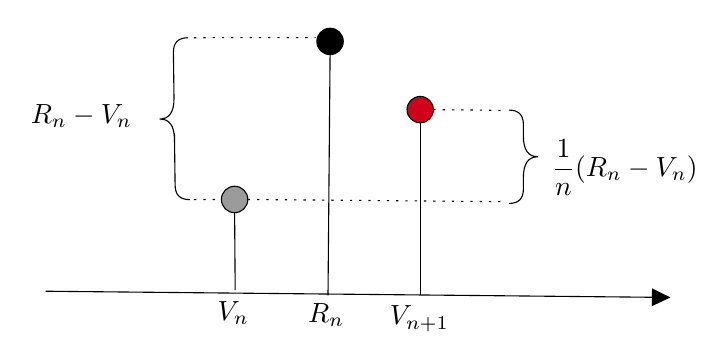
\begin{tikzpicture}[x=0.75pt,y=0.75pt,yscale=-1,xscale=1]
					%uncomment if require: \path (0,390); %set diagram left start at 0, and has height of 390
					
					%Shape: Circle [id:dp8823658462262833] 
					\draw  [fill={rgb, 255:red, 0; green, 0; blue, 0 }  ,fill opacity=1 ] (210.07,88.79) .. controls (210.07,85.27) and (212.92,82.43) .. (216.43,82.43) .. controls (219.94,82.43) and (222.79,85.27) .. (222.79,88.79) .. controls (222.79,92.3) and (219.94,95.14) .. (216.43,95.14) .. controls (212.92,95.14) and (210.07,92.3) .. (210.07,88.79) -- cycle ;
					%Straight Lines [id:da4015400832093903] 
					\draw    (216.43,95.14) -- (215.43,211.14) ;
					
					%Straight Lines [id:da97617721159805] 
					\draw    (170.43,171.29) -- (170.71,208.64) ;
					%Shape: Circle [id:dp1419005313510331] 
					\draw  [fill={rgb, 255:red, 155; green, 155; blue, 155 }  ,fill opacity=1 ] (164.07,164.93) .. controls (164.07,161.42) and (166.92,158.57) .. (170.43,158.57) .. controls (173.94,158.57) and (176.79,161.42) .. (176.79,164.93) .. controls (176.79,168.44) and (173.94,171.29) .. (170.43,171.29) .. controls (166.92,171.29) and (164.07,168.44) .. (164.07,164.93) -- cycle ;
					%Straight Lines [id:da8939405937546931] 
					\draw    (79.43,209.14) -- (377.43,212.11) ;
					\draw [shift={(380.43,212.14)}, rotate = 180.57] [fill={rgb, 255:red, 0; green, 0; blue, 0 }  ][line width=0.08]  [draw opacity=0] (8.93,-4.29) -- (0,0) -- (8.93,4.29) -- cycle    ;
					%Shape: Circle [id:dp12276156906197633] 
					\draw  [fill={rgb, 255:red, 208; green, 2; blue, 27 }  ,fill opacity=1 ] (253.5,121.64) .. controls (253.5,118.13) and (256.35,115.29) .. (259.86,115.29) .. controls (263.37,115.29) and (266.21,118.13) .. (266.21,121.64) .. controls (266.21,125.15) and (263.37,128) .. (259.86,128) .. controls (256.35,128) and (253.5,125.15) .. (253.5,121.64) -- cycle ;
					%Straight Lines [id:da6832821685568764] 
					\draw    (259.86,128) -- (259.86,211) ;
					%Straight Lines [id:da3728032563114083] 
					\draw  [dash pattern={on 0.84pt off 2.51pt}]  (150.86,165) -- (164.07,164.93) ;
					%Straight Lines [id:da16497485961263725] 
					\draw  [dash pattern={on 0.84pt off 2.51pt}]  (150.86,87) -- (209.43,86.93) ;
					%Shape: Brace [id:dp9955993231598876] 
					\draw   (147.86,87) .. controls (143.19,87.06) and (140.89,89.42) .. (140.95,94.09) -- (141.23,116.09) .. controls (141.31,122.76) and (139.02,126.12) .. (134.36,126.18) .. controls (139.02,126.12) and (141.39,129.42) .. (141.48,136.09)(141.44,133.09) -- (141.76,158.09) .. controls (141.82,162.76) and (144.18,165.06) .. (148.85,165) ;
					%Straight Lines [id:da7322997374980948] 
					\draw  [dash pattern={on 0.84pt off 2.51pt}]  (176.79,164.93) -- (300.71,166) ;
					%Shape: Brace [id:dp1665700630787652] 
					\draw   (302.57,166.86) .. controls (307.24,166.86) and (309.57,164.53) .. (309.57,159.86) -- (309.57,154.36) .. controls (309.57,147.69) and (311.9,144.36) .. (316.57,144.36) .. controls (311.9,144.36) and (309.57,141.03) .. (309.57,134.36)(309.57,137.36) -- (309.57,128.86) .. controls (309.57,124.19) and (307.24,121.86) .. (302.57,121.86) ;
					%Straight Lines [id:da5111771395055766] 
					\draw  [dash pattern={on 0.84pt off 2.51pt}]  (266.21,121.64) -- (299.71,122) ;
					
					% Text Node
					\draw (161,213) node [anchor=north west][inner sep=0.75pt]   [align=left] {$\displaystyle V_{n}$};
					% Text Node
					\draw (71,118) node [anchor=north west][inner sep=0.75pt]   [align=left] {$\displaystyle R_{n} -V_{n}$};
					% Text Node
					\draw (204.57,214) node [anchor=north west][inner sep=0.75pt]   [align=left] {$\displaystyle R_{n}$};
					% Text Node
					\draw (244,215) node [anchor=north west][inner sep=0.75pt]   [align=left] {$\displaystyle V_{n+1}$};
					% Text Node
					\draw (322,135) node [anchor=north west][inner sep=0.75pt]   [align=left] {$\displaystyle \frac{1}{n}( R_{n} -V_{n})$};
					
					
				\end{tikzpicture}
				
				
				
				\hspace{1.5cm}
				
				\tikzset{every picture/.style={line width=0.75pt}} %set default line width to 0.75pt        
				
				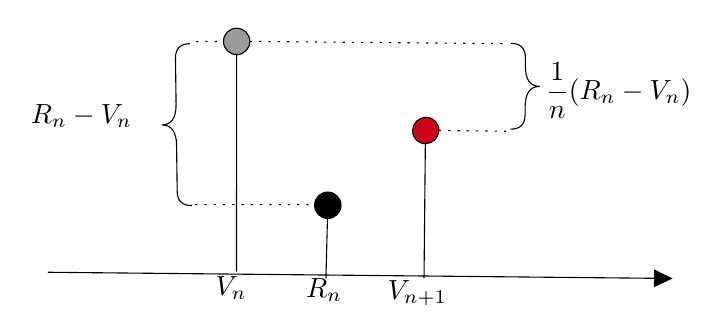
\begin{tikzpicture}[x=0.75pt,y=0.75pt,yscale=-1,xscale=1]
					%uncomment if require: \path (0,300); %set diagram left start at 0, and has height of 300
					
					%Shape: Circle [id:dp4484948614161621] 
					\draw  [fill={rgb, 255:red, 0; green, 0; blue, 0 }  ,fill opacity=1 ] (294.98,130.86) .. controls (294.98,127.35) and (297.82,124.51) .. (301.33,124.51) .. controls (304.84,124.51) and (307.69,127.35) .. (307.69,130.86) .. controls (307.69,134.38) and (304.84,137.22) .. (301.33,137.22) .. controls (297.82,137.22) and (294.98,134.38) .. (294.98,130.86) -- cycle ;
					%Straight Lines [id:da2819688419673383] 
					\draw    (301.33,130.86) -- (300.43,166.14) ;
					%Straight Lines [id:da36211637573626887] 
					\draw    (257.43,58.29) -- (257.33,162.86) ;
					%Shape: Circle [id:dp5979619034484167] 
					\draw  [fill={rgb, 255:red, 155; green, 155; blue, 155 }  ,fill opacity=1 ] (251.07,51.93) .. controls (251.07,48.42) and (253.92,45.57) .. (257.43,45.57) .. controls (260.94,45.57) and (263.79,48.42) .. (263.79,51.93) .. controls (263.79,55.44) and (260.94,58.29) .. (257.43,58.29) .. controls (253.92,58.29) and (251.07,55.44) .. (251.07,51.93) -- cycle ;
					%Straight Lines [id:da7251288276270931] 
					\draw    (166.43,163.14) -- (464.43,166.11) ;
					\draw [shift={(467.43,166.14)}, rotate = 180.57] [fill={rgb, 255:red, 0; green, 0; blue, 0 }  ][line width=0.08]  [draw opacity=0] (8.93,-4.29) -- (0,0) -- (8.93,4.29) -- cycle    ;
					%Shape: Circle [id:dp9166215407051872] 
					\draw  [fill={rgb, 255:red, 208; green, 2; blue, 27 }  ,fill opacity=1 ] (342.14,94.84) .. controls (342.23,91.33) and (345.16,88.48) .. (348.67,88.48) .. controls (352.18,88.48) and (354.95,91.33) .. (354.86,94.84) .. controls (354.77,98.35) and (351.84,101.2) .. (348.33,101.2) .. controls (344.82,101.2) and (342.05,98.35) .. (342.14,94.84) -- cycle ;
					%Straight Lines [id:da19061248181682844] 
					\draw    (348.33,101.2) -- (347.69,166) ;
					%Straight Lines [id:da9603240712238956] 
					\draw  [dash pattern={on 0.84pt off 2.51pt}]  (237.86,52) -- (251.07,51.93) ;
					%Straight Lines [id:da44219430731016907] 
					\draw  [dash pattern={on 0.84pt off 2.51pt}]  (237.4,130.58) -- (295.98,130.51) ;
					%Shape: Brace [id:dp9158682145980315] 
					\draw   (234.86,53) .. controls (230.19,53.06) and (227.89,55.42) .. (227.95,60.09) -- (228.23,82.09) .. controls (228.31,88.76) and (226.02,92.12) .. (221.36,92.18) .. controls (226.02,92.12) and (228.39,95.42) .. (228.48,102.09)(228.44,99.09) -- (228.76,124.09) .. controls (228.82,128.76) and (231.18,131.06) .. (235.85,131) ;
					%Straight Lines [id:da14415284974266251] 
					\draw  [dash pattern={on 0.84pt off 2.51pt}]  (263.79,51.93) -- (387.71,53) ;
					%Shape: Brace [id:dp5965412064250464] 
					\draw   (389.33,94.2) .. controls (394,94.23) and (396.34,91.91) .. (396.37,87.24) -- (396.39,83.57) .. controls (396.43,76.9) and (398.78,73.58) .. (403.45,73.61) .. controls (398.78,73.58) and (396.47,70.24) .. (396.51,63.57)(396.49,66.57) -- (396.53,59.9) .. controls (396.56,55.23) and (394.24,52.89) .. (389.57,52.86) ;
					%Straight Lines [id:da6655545338004027] 
					\draw  [dash pattern={on 0.84pt off 2.51pt}]  (354.86,94.84) -- (388.36,95.2) ;
					
					% Text Node
					\draw (246,164) node [anchor=north west][inner sep=0.75pt]   [align=left] {$\displaystyle V_{n}$};
					% Text Node
					\draw (157,81) node [anchor=north west][inner sep=0.75pt]   [align=left] {$\displaystyle R_{n} -V_{n}$};
					% Text Node
					\draw (289.57,165) node [anchor=north west][inner sep=0.75pt]   [align=left] {$\displaystyle R_{n}$};
					% Text Node
					\draw (329,166) node [anchor=north west][inner sep=0.75pt]   [align=left] {$\displaystyle V_{n+1}$};
					% Text Node
					\draw (405,61) node [anchor=north west][inner sep=0.75pt]   [align=left] {$\displaystyle \frac{1}{n}( R_{n} -V_{n})$};
					
					
				\end{tikzpicture}		
		}}
		
		
		
		\item \key{De forma general}, se puede ver de la siguiente manera:
		
		\centerline{\normalsize  $\color{violet} {Nuevo Estimado} = {Viejo Estimado} + {Tama\text{\itñ}o del Paso} \cdot \left( {Objetivo} - {Viejo Estimado} \right).$}
		
		\begin{itemize}
			\item Para obtener una nueva estimación para un objetivo, usamos la \textbf{estimación antigua}. 
			
			\item[]\qquad \key{Error de la estimación:} $\color{violet} \left( {Objetivo} - {Viejo Estimado} \right)$ 
			
			\item También usamos  un \textbf{tamaño de paso}.
			\item[]\qquad \key{El tamaño de paso establece la dirección hacia el objetivo, $\alpha$.}
			
			\item \textbf{Ejemplo} para el promedio incremental.
			
			\begin{itemize}
				\item Para obtener una nueva estimación para un promedio,  usamos el promedio antiguo y un tamaño de paso.
				\item El parámetro  $\color{violet} \alpha=Tama\text{\itñ}o del Paso = 1/n$ cambia de paso de tiempo a paso de tiempo.
				\item Error de la estimación: $\color{violet} \left( {Objetivo} - {Viejo Estimado} \right)$ 
				\item $\alpha_n=1/n$ establece la dirección hacia el objetivo.
			\end{itemize}
		\end{itemize}
		
	\end{itemize}
	
\end{frame}



%%%%%%%%%%%%%%%%%
%%%%%%%%%%%%%%%%%
\begin{frame}{Comparación entre Técnicas de Aprendizaje por Refuerzo.}
	
	\large
	\centering
	\begin{tabularx}{\textwidth}{c|Y} 
		\textbf{Técnica}    & \textbf{Euación de Bellman} y su \textbf{Fórmula de Aproximación} \\ \hline \\
		Monte Carlo         & ~ ~ ~ ~ ~ ~ $v_\pi(s) = \mathbb{E}[{\color{blue} G_t} \mid S_t = s]$  \newline $V(S_t) \gets V(S_t) + \alpha [ {\color{reddark} G_t} - V(S_t)]$ \\ \\
		
		TD(0)               & ~ ~ $v_\pi(s) = \mathbb{E}[{\color{blue} R_{t+1} + \gamma v_\pi(S_{t+1}) } \mid S_t = s]$ 
		\newline $V(S_t) \gets V(S_t) + \alpha [{\color{reddark} R_{t+1} + \gamma V(S_{t+1})} - V(S_t)]$ \\ \\
		
		SARSA               & $q_\pi(s, a) = \mathbb{E}[{\color{blue} R_{t+1} + \gamma q_\pi(S_{t+1}, A_{t+1})} \mid S_t = s, A_t = a]$ 
		\newline $Q(S_t, A_t) \gets Q(S_t, A_t) + \alpha [{\color{reddark} R_{t+1} + \gamma Q(S_{t+1}, A_{t+1})} - Q(S_t, A_t)]$ \\ \\
		
		Q-Learning          & $q_*(s, a) = \mathbb{E}[{\color{blue} R_{t+1} + \gamma \max_{a'} q_*(S_{t+1}, a') } \mid S_t = s, A_t = a]$ 
		\newline $Q(S_t, A_t) \gets Q(S_t, A_t) + \alpha [{\color{reddark} R_{t+1} + \gamma \max_a Q(S_{t+1}, a)} - Q(S_t, A_t)]$ \\  \\
		
		Expected SARSA      & $q_\pi(s, a) = \mathbb{E}[{\color{blue} R_{t+1} + \gamma \sum_{a'} \pi(a' \mid S_{t+1}) q_\pi(S_{t+1}, a')}]$ 
		\newline {\small  $Q(S_t, A_t) \gets Q(S_t, A_t) + \alpha \left[{\color{reddark} R_{t+1} + \gamma \sum_{a'} \pi(a' \mid S_{t+1}) Q(S_{t+1}, a')} - Q(S_t, A_t)\right]$} \\
	\end{tabularx}

\end{frame}





%%%%%%%%%%%%%%%%%%%%%%%%%%%%%%%%%%%%%%%%%%%%%%%%%%%%%%%%%%%%%%%%%%%%
%%%%%%%%%%%%%%%%%%%%%%%%%%%%%%%%%%%%%%%%%%%%%%%%%%%%%%%%%%%%%%%%%%%%

\section{Predicción}



%%%%%%%%%%%%%%%%%%%%%%%%%%%%%%%%%%%%%%%%%%%%%%%%%%%%%%%%%%%%%%%%%%%%
%%%%%%%%%%%%%%%%%%%%%%%%%%%%%%%%%%%%%%%%%%%%%%%%%%%%%%%%%%%%%%%%%%%%

\subsection{Diferencias Temporales a un Paso: TD(0)}



%%%%%%%%%%%%%%%%%%%%%%%%%%%%%%%%%%
%%%%%%%%%%%%%%%%%%%%%%%%%%%%%%%%%%

\begin{frame}{Monte Carlo $\alpha$-constante y TD(0)}
	
\begin{itemize}
%	\item Recordemos lo siguiente:
%	
%	\begin{align}
%		v_\pi(s) &\stackrel{\cdot}{=} \mathbb{E}_\pi[G_t | S_t = s] \label{eq:1} \\
%%		&= \mathbb{E}_\pi[R_{t+1} + \gamma G_{t+1} | S_t = s] \quad \nonumber (\text{de } (3.9)) \\
%%		&= \mathbb{E}_\pi[R_{t+1} + \gamma v^\pi(S_{t+1}) | S_t = s] \, . \label{eq:2}
%	\end{align}
%		
		
	\item En \key{Monte Carlo}  nuestro objetivo es calcular: $\ds v_\pi(s) \stackrel{\cdot}{=} \mathbb{E}_\pi[G_t | S_t = s] $
	
	%\item Ley de los grandes números: $\ds\mathbb{E}_\pi[G_t|s_t=s] \approx  \frac{1}{N} \sum_{i=1}^{N} G_t^{(i)}$.
		
	\item Pero al no tener modelo, \key{calculamos un promedio}: $\ds v_\pi(s) \stackrel{\cdot}{=} \mathbb{E}_\pi[{\color{magenta} G_t} | S_t = s] \approx \frac{1}{N} \sum_{i=1}^{N} G_t^{(i)}$
	

		
	\item Si aplicamos el \key{cálculo incremental} (para todos los estados - aplicado en predicción MC):
		\begin{itemize}
			\item  $N(S_t) \leftarrow N(S_t) + 1$
			\item  $\ds V(S_t) \gets V(S_t) + \frac{1}{N(S_t)} \Big({\color{magenta} G_t} - V(S_t)\Big)$ 
		\end{itemize}
	
	\item \key{MC con $\alpha$ constante}: $V(S_t) \gets V(S_t) + \alpha \left({\color{magenta}  G_t} - V(S_t)\right)$
	
	
	\item Sabemos que: 
	
	{\large $v_\pi(s) \stackrel{\cdot}{=} \mathbb{E}_\pi[{\color{magenta} G_t} | S_t = s] = \mathbb{E}_\pi[R_{t+1} + \gamma G_{t+1} | S_t = s] = \mathbb{E}_\pi[{\color{red} R_{t+1} + \gamma v_\pi(S_{t+1})} | S_t = s] $}
	
	\item \key{TD(0)}: $V(S_t) \gets V(S_t) + \alpha \left({\color{red} R_{t+1} + \gamma V(S_{t+1})} - V(S_t)\right)$
		\hfill \key{Error DT}: $\delta_t={\color{red} R_{t+1} + \gamma V(S_{t+1})} - V(S_t)$
	
	\item Las diferencias \textbf{de forma gráfica}:
	\end{itemize}

	


	\centerline{\scalebox{.6}{
	
	
	
	
	\tikzset{every picture/.style={line width=0.75pt}} %set default line width to 0.75pt        
	
	
	
	
	\tikzset{every picture/.style={line width=0.75pt}} %set default line width to 0.75pt        
	
	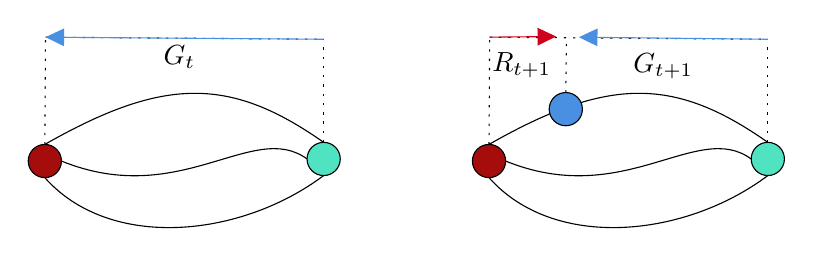
\begin{tikzpicture}[x=0.75pt,y=0.75pt,yscale=-1,xscale=1]
		%uncomment if require: \path (0,300); %set diagram left start at 0, and has height of 300
		
		%Shape: Circle [id:dp3629901772445876] 
		\draw  [fill={rgb, 255:red, 165; green, 12; blue, 12 }  ,fill opacity=1 ] (33,90) .. controls (33,85.58) and (36.58,82) .. (41,82) .. controls (45.42,82) and (49,85.58) .. (49,90) .. controls (49,94.42) and (45.42,98) .. (41,98) .. controls (36.58,98) and (33,94.42) .. (33,90) -- cycle ;
		%Curve Lines [id:da5799450866899267] 
		\draw    (41,82) .. controls (98.33,49.33) and (130.33,49.33) .. (175.33,81) ;
		%Curve Lines [id:da27761182884727] 
		\draw    (49,90) .. controls (106.33,113.33) and (141.33,70) .. (167.33,89) ;
		%Curve Lines [id:da4716883199243478] 
		\draw    (41,98) .. controls (72.33,133.33) and (135.33,127) .. (175.33,97) ;
		%Straight Lines [id:da39718368386382163] 
		\draw  [dash pattern={on 0.84pt off 2.51pt}]  (41,82) -- (41.33,30.33) ;
		%Shape: Circle [id:dp8611307374285766] 
		\draw  [fill={rgb, 255:red, 80; green, 227; blue, 194 }  ,fill opacity=1 ] (167.33,89) .. controls (167.33,84.58) and (170.92,81) .. (175.33,81) .. controls (179.75,81) and (183.33,84.58) .. (183.33,89) .. controls (183.33,93.42) and (179.75,97) .. (175.33,97) .. controls (170.92,97) and (167.33,93.42) .. (167.33,89) -- cycle ;
		%Straight Lines [id:da2727270077877346] 
		\draw  [dash pattern={on 0.84pt off 2.51pt}]  (175.33,81) -- (175.33,31.33) ;
		%Straight Lines [id:da40929111486693004] 
		\draw  [dash pattern={on 0.84pt off 2.51pt}]  (41.33,30.33) -- (175.33,31.33) ;
		%Shape: Circle [id:dp2997563872374802] 
		\draw  [fill={rgb, 255:red, 165; green, 12; blue, 12 }  ,fill opacity=1 ] (247,90) .. controls (247,85.58) and (250.58,82) .. (255,82) .. controls (259.42,82) and (263,85.58) .. (263,90) .. controls (263,94.42) and (259.42,98) .. (255,98) .. controls (250.58,98) and (247,94.42) .. (247,90) -- cycle ;
		%Curve Lines [id:da7367805598229356] 
		\draw    (255,82) .. controls (312.33,49.33) and (344.33,49.33) .. (389.33,81) ;
		%Curve Lines [id:da23044500261217538] 
		\draw    (263,90) .. controls (320.33,113.33) and (355.33,70) .. (381.33,89) ;
		%Curve Lines [id:da7127225622960531] 
		\draw    (255,98) .. controls (286.33,133.33) and (349.33,127) .. (389.33,97) ;
		%Straight Lines [id:da2915631263334295] 
		\draw  [dash pattern={on 0.84pt off 2.51pt}]  (255,82) -- (255.33,30.33) ;
		%Shape: Circle [id:dp6390948739369489] 
		\draw  [fill={rgb, 255:red, 80; green, 227; blue, 194 }  ,fill opacity=1 ] (381.33,89) .. controls (381.33,84.58) and (384.92,81) .. (389.33,81) .. controls (393.75,81) and (397.33,84.58) .. (397.33,89) .. controls (397.33,93.42) and (393.75,97) .. (389.33,97) .. controls (384.92,97) and (381.33,93.42) .. (381.33,89) -- cycle ;
		%Straight Lines [id:da9837461798140881] 
		\draw  [dash pattern={on 0.84pt off 2.51pt}]  (389.33,81) -- (389.33,31.33) ;
		%Straight Lines [id:da6104066092789611] 
		\draw  [dash pattern={on 0.84pt off 2.51pt}]  (255.33,30.33) -- (389.33,31.33) ;
		%Shape: Circle [id:dp389357216883474] 
		\draw  [fill={rgb, 255:red, 74; green, 144; blue, 226 }  ,fill opacity=1 ] (284,65) .. controls (284,60.58) and (287.58,57) .. (292,57) .. controls (296.42,57) and (300,60.58) .. (300,65) .. controls (300,69.42) and (296.42,73) .. (292,73) .. controls (287.58,73) and (284,69.42) .. (284,65) -- cycle ;
		%Straight Lines [id:da048343594880042584] 
		\draw  [dash pattern={on 0.84pt off 2.51pt}]  (292,57) -- (292.33,32) ;
		%Straight Lines [id:da7278991554861851] 
		\draw [color={rgb, 255:red, 74; green, 144; blue, 226 }  ,draw opacity=1 ]   (175.33,31.33) -- (44.33,30.36) ;
		\draw [shift={(41.33,30.33)}, rotate = 0.43] [fill={rgb, 255:red, 74; green, 144; blue, 226 }  ,fill opacity=1 ][line width=0.08]  [draw opacity=0] (8.93,-4.29) -- (0,0) -- (8.93,4.29) -- cycle    ;
		%Straight Lines [id:da43176557408969063] 
		\draw [color={rgb, 255:red, 74; green, 144; blue, 226 }  ,draw opacity=1 ]   (389.33,31.33) -- (301.33,30.37) ;
		\draw [shift={(298.33,30.33)}, rotate = 0.63] [fill={rgb, 255:red, 74; green, 144; blue, 226 }  ,fill opacity=1 ][line width=0.08]  [draw opacity=0] (8.93,-4.29) -- (0,0) -- (8.93,4.29) -- cycle    ;
		%Straight Lines [id:da42075719468980344] 
		\draw [color={rgb, 255:red, 208; green, 2; blue, 27 }  ,draw opacity=1 ]   (255.33,30.33) -- (284.33,30.03) ;
		\draw [shift={(287.33,30)}, rotate = 179.4] [fill={rgb, 255:red, 208; green, 2; blue, 27 }  ,fill opacity=1 ][line width=0.08]  [draw opacity=0] (8.93,-4.29) -- (0,0) -- (8.93,4.29) -- cycle    ;
		
		% Text Node
		\draw (97,33) node [anchor=north west][inner sep=0.75pt]   [align=left] {$\displaystyle G_{t}$};
		% Text Node
		\draw (323.33,36.83) node [anchor=north west][inner sep=0.75pt]   [align=left] {$\displaystyle G_{t+1}$};
		% Text Node
		\draw (255.33,36.33) node [anchor=north west][inner sep=0.75pt]   [align=left] {$\displaystyle R_{t+1}$};
		
		
	\end{tikzpicture}
	}}

\end{frame}



%%%%%%%%%%%%%%%%%%%%%%%%%%%%%%%%%%
%%%%%%%%%%%%%%%%%%%%%%%%%%%%%%%%%%
\begin{frame}{TD(0) tabular para estimar $v_\pi$}{\cite{Sutton2018}}
	
	
\begin{algorithm}[H]
	\caption{TD(0) tabular para estimar $v_\pi$}
	\includegraphics[width=\textwidth]{fig/tabularTD0}
\end{algorithm}
	

\note{
	\begin{itemize}
		\item Aquí se muestra la versión de \textit{Diferencias Temporales de un paso} o TD(0)
		
		\item El proceso es simple:
			\begin{itemize}
				\item \key{Nos dan la política} que queramos evaluar y el tamaño de paso.
				\item Damos \key{valores arbitrarios a los valores de estados salvo} al estado terminal que le damos un valor de 0.
				\item Entonces \key{generamos episodios sin fin}.
				\item Para cada episodio \key{empezamos en un estado S} y nos \textbf{movemos} en el entorno \textbf{según diga la política}.
				\item \key{Para cada acción} que tomemos abandonamos nuestro estado actual S para ir a un estado futuro S', observamos la recompensa R y \key[red]{actualizamos el estado S que abandonamos} de acuerdo a la suma del valor que ya tenía y un porcentaje $\alpha$ del error de la estimación.
			\end{itemize}
			
		
		\item  Ya que TD(0) \key{se basa su actualización en parte en una estimación existente,} decimos que es un método de \textit{bootstrapping}
	\end{itemize}
	\fin
}

\end{frame}





%%%%%%%%%%%%%%%%%%%%%%%%%%%%%%%%%%
%%%%%%%%%%%%%%%%%%%%%%%%%%%%%%%%%%

\begin{frame}[label={frame:SizeParam}]{Ventajas de los Métodos de Predicción TD}
		
\begin{itemize}
	\item Los \key{métodos TD} tienen una ventaja \key{sobre los métodos de Programación Dinámica} (DP) en que \textbf{no requieren un modelo del entorno}, de sus recompensas y distribuciones de probabilidad del siguiente estado.
	
	\item Los \key{métodos TD} tienen una ventaja \key{sobre los métodos de Monte Carlo} (MC) en que están \textbf{naturalmente implementados en línea} (on-line), de forma completamente incremental.
	
	\item \key{Los métodos TD convergen}. Para cualquier política fija \(\pi\), con \(TD(0)\) se garantiza que $\ds \lim_{t \to \infty} V_t(s) = v_\pi(s)$  con \textbf{probabilidad 1} si el parámetro de tamaño de paso \textbf{disminuye} de acuerdo con las \key[red]{condiciones de aproximación estocástica} (Condiciones de Robbins-Monro) para la tasa de aprendizaje $\alpha_n$:
	
	\centerline{$\ds\sum_{n=1}^\infty \alpha_n(a) = \infty \quad \text{y} \quad \sum_{n=1}^\infty \alpha_n^2(a) < \infty.$}
	
	\item \key{En la práctica}, los métodos TD generalmente han mostrado una \textbf{velocidad de convergencia más rápida que los métodos Monte Carlo constante-\(\alpha\)} en tareas estocásticas; pero no está demostrado.
\end{itemize}
\end{frame}




%%%%%%%%%%%%%%%%%%%%%%%%%%%%%%%%%%
%%%%%%%%%%%%%%%%%%%%%%%%%%%%%%%%%%

\begin{frame}{Ejemplo: Paseo Aleatorio}

	
	\begin{center}
		\includegraphics[width=0.8\textwidth]{fig/randomWalk}
	
	\begin{columns}
\begin{column}{.5\textwidth}

\textbf{Ejemplo de Episodio:} $C, 0, B, 0, C, 0, D, 0, E, 1$

\footnotesize	
\hfil \(v(A) = \frac{1}{6}\),
		\(v(B) = \frac{2}{6}\),
		\(v(C) = \frac{3}{6}\),
		
\hfil \(v(D) = \frac{4}{6}\),
		\(v(E) = \frac{5}{6}\).
\end{column}
\begin{column}{.5\textwidth}
\textbf{Ecuaciones de Bellman:}  $v(s) = \sum_{s'} P(s' \mid s) \left[ R(s, s') + \gamma v(s') \right]$
\footnotesize

\(v(A) = 0.5 \cdot v(B)\),
				\(v(B) = 0.5 \cdot v(A) + 0.5 \cdot v(C)\),
				\(v(C) = 0.5 \cdot v(B) + 0.5 \cdot v(D)\),
				\(v(D) = 0.5 \cdot v(C) + 0.5 \cdot v(E)\),
				\(v(E) = 0.5 \cdot v(D) + 0.5\).
\end{column}
\end{columns}

		
		\vfill
		\includegraphics[width=0.75\textwidth]{fig/randomWalk2}
	\end{center}
	

\end{frame}









%%%%%%%%%%%%%%%%%%%%%%%%%%%%%%%%%%%%%%%%%%%%%%%%%%%%%%%%%%%%%%%%%%%%
%%%%%%%%%%%%%%%%%%%%%%%%%%%%%%%%%%%%%%%%%%%%%%%%%%%%%%%%%%%%%%%%%%%%

\subsection{Optimalidad de TD(0) - Por lotes}




%%%%%%%%%%%%%%%%%%%%%%%%%%%%%%%%%%
%%%%%%%%%%%%%%%%%%%%%%%%%%%%%%%%%%
\begin{frame}{Actualización por lotes (Batch updating)}

	
\begin{itemize}
	\item Observa las expresiones:
	\centerline{$	V(S_t) \gets V(S_t) + \alpha \left({\color{reddark} G_t} - V(S_t)\right) \hfil
		V(S_t) \gets V(S_t) + \alpha \left({\color{reddark} R_{t+1} + \gamma V(S_{t+1})} - V(S_t)\right)$}
		
	\item ¿Por qué no usar un lote (conjunto de muestras) en vez de solo una muestra?
	
	\item Batch updating (ver \cite{lange2012batch} para más técnicas):
%		\begin{enumerate}
%			\item Genera un lote
%			\item Calcular los $\delta_t(s)=Error_t$ para cada estado visitado no terminal.
%			\item Actualizar la función de valor (solo una vez) por la suma de todos los incrementos.
%			$V(s) \gets V(s) + \alpha \sum_t \delta_t(s)$
%			\item Si no converge, volver a 1.
%		\end{enumerate}
	

\item Para \key{TD(0) con $\alpha$ constante}

\scalebox{0.7}{
	\begin{minipage}{0.9\textwidth}
		\begin{algorithm}[H]
			\caption{Diferencias Temporales por Lotes con Tasa de Aprendizaje Constante}
			\begin{algorithmic}[1]
				\REQUIRE  $\alpha$ (tasa de aprendizaje constante), $\gamma$ (factor de descuento), $\pi$ (política)
				\STATE \textbf{Inicializar} $V(s) \leftarrow 0$ para todo $s \in S$
				\WHILE{no convergencia}
				\STATE \textbf{Recopilar} un lote de transiciones $\mathcal{D} = \{(s_t, A_t, R_{t+1}, s_{t+1})\}$ a partir de episodios aleatorios.

				\FOR{cada transición $(s_t, A_t, R_{t+1}, s_{t+1})$ en $\mathcal{D}$}
				\STATE \textbf{Calcular} el error de TD: $\delta(s_t) \gets R_{t+1} + \gamma V(s_{t+1}) - V(s_t)$
				\STATE \textbf{Actualizar} la función de valor: $V(s_t) \leftarrow V(s_t) + \alpha \delta(s_t)$
				\ENDFOR \quad \textit{Repetir el \textbf{for} hasta que ``converga'' si solo hay un lote}
				\STATE \textbf{Verificar} convergencia de $V(s)$ (p.e. $\max_{s} |V(s) - V_{\text{anterior}}(s)|<\epsilon$  entre 2 lotes consecutivos)
				\ENDWHILE
			\end{algorithmic}
		\end{algorithm}
\end{minipage}} 
\begin{minipage}{.3\textwidth}
	\begin{itemize} \scriptsize
		\item \key{Usa TD(0) sin lotes} si…
		
		Necesitas respuestas rápidas y en línea.
		Estás trabajando con sistemas en tiempo real. Hay flujo continuo de datos.
		El entorno cambia constantemente.
		
		
		\item \key{Usa TD(0) por Lotes} si…
		
		Quieres estabilidad en el aprendizaje.
		Tienes un conjunto limitado de datos (aprendizaje fuera de línea).
		Quieres mejorar la eficiencia computacional en modelos grandes.
		
	\end{itemize}
	
	
\end{minipage}

\item Para \key{MC  $\alpha$-constan}t, actualizar \( V(s) \) como el \textbf{promedio de todos los retornos observados} en el lote:

\centerline{$
	V(s) \leftarrow V(s) + \alpha \cdot \left( {\color{reddark} \frac{1}{n(s)} \sum G(s)} - V(s) \right)
	$}

\begin{itemize}
	\item \( n(s) \) es el número de veces que se ha visitado \( s \) en el lote.
\end{itemize}

\end{itemize}
\end{frame}




%%%%%%%%%%%%%%%%%%%%%%%%%%%%%%%%%%
%%%%%%%%%%%%%%%%%%%%%%%%%%%%%%%%%%
\begin{frame}{Optimalidad de TD(0)}
	\key{Actualización por lotes (Batch updating):}
	\begin{itemize}
		\item \key{TD(0)  converge determinísticamente} a una única solución independiente del parámetro de tamaño de paso, \(\alpha\), siempre que \(\alpha\) sea suficientemente pequeño.
		\item El método de \key{Monte Carlo} constante-\(\alpha\) también \key{converge determinísticamente} bajo las mismas condiciones, pero a una solución diferente.
	\end{itemize}
	
\vfill 

	\textbf{Ejemplo:} \textit{Paseo Aleatorio}

\centerline{\includegraphics[width=0.5\textwidth]{fig/randomWalk}; } 

\centerline{\raisebox{2cm}{\scriptsize$\ds \text{RMS error} = \sqrt{\frac{1}{|S|} \sum_{s \in S} \left( V(s) - v_\pi(s) \right)^2 }$} ~ ~ \includegraphics[width=0.4\textwidth]{fig/learning_curves}}

\end{frame}




%%%%%%%%%%%%%%%%%%%%%%%%%%%%%%%%%%
%%%%%%%%%%%%%%%%%%%%%%%%%%%%%%%%%%
\begin{frame}{Optimalidad de TD(0)}{Adivina adivinanza ....}
\begin{itemize}
	\item Considera un \textbf{Proceso de \key{Recompensa} de Markov} desconocido (no tiene acciones).
	
	\item Supón que \textbf{observas los siguientes ocho episodios}:
	
	\centerline{\begin{tabular}{lll}
		A, 0, B, 0  & & B, 1 \\
		B, 1 &  & B, 1 \\
		B, 1 & & B, 1 \\
		B, 1 & & B, 0
	\end{tabular}}
	
	\item ¿Cuánto debería ser el \key{valor esperado del retorno} para cada estado?
	
	\centerline{\begin{tabular}{lll}
		\textbf{MC} & & \textbf{TD(0)} \\ \hline
		v(B)=6/8=3/4 &  & v(B) = 3/4 \\
		v(A)=0 &  & v(A) = 3/4 \\
		\end{tabular}}	 
	
	\item ¿Por qué?
	
	\centerline{\includegraphics[width=0.25\textwidth]{fig/YouArepredictor}; } 
\end{itemize}
\end{frame}





%%%%%%%%%%%%%%%%%%%%%%%%%%%%%%%%%%
%%%%%%%%%%%%%%%%%%%%%%%%%%%%%%%%%%
\begin{frame}{\S Optimalidad de TD(0)}{Resultados Finales}

\begin{itemize}
	\item Los métodos \key{Monte Carlo por lotes} siempre encuentran las estimaciones que \key{minimizan} el \textbf{error cuadrático medio en el conjunto de entrenamiento}.
	
	\item \key{Batch TD(0)} siempre encuentra las estimaciones que serían exactamente correctas para el \textbf{modelo de máxima verosimilitud del proceso de Markov}:
	\begin{itemize}
		\item Una estimación de máxima verosimilitud de un parámetro es el \textbf{valor del parámetro cuya probabilidad de generar los datos es la mayor}. $\hat{\theta} = \arg \max_{\theta} P(\text{Datos} \mid \theta)$
		
		\item La \textbf{probabilidad estimada de transición de \( i \) a \( j \)} es el {promedio de transiciones observadas de \( i \) a \( j \)}, 
		
		\centerline{$P(i \to j) = \frac{\text{Número de transiciones observadas de } i \text{ a } j}{\text{Número total de transiciones desde } i}$}
		
		\item La \textbf{recompensa esperada} asociada es el promedio de las recompensas observadas en esas transiciones.
		
		\centerline{$R(i \to j) = \frac{\text{Suma de recompensas observadas en las transiciones de } i \text{ a } j}{\text{Número de transiciones observadas de } i \text{ a } j}$}
		
	\end{itemize}
	
	\item Dado este modelo, podemos calcular la \key{estimación de la función de valor que sería exactamente correcta si el modelo fuera exactamente correcto}.
	
	\centerline{$V(s) = \sum_{j \in S} P(s \to j) \left[ R(s \to j) + \gamma V(j) \right]$}
	
	\begin{itemize}
		\item Esto se llama la \key{estimación de equivalencia a certeza}, porque es equivalente a asumir que la estimación del proceso subyacente se conocía con certeza en lugar de ser aproximada.
	\end{itemize}
	
	\item \key{Batch TD(0) converge a la estimación de equivalencia a certeza}.
\end{itemize}
\end{frame}




%%%%%%%%%%%%%%%%%%%%%%%%%%%%%%%%%%%%%%%%%%%%%%%%%%%%%%%%%%%%%%%%%%%%
%%%%%%%%%%%%%%%%%%%%%%%%%%%%%%%%%%%%%%%%%%%%%%%%%%%%%%%%%%%%%%%%%%%%

\section{Control}

%%%%%%%%%%%%%%%%%%%%%%%%%%%%%%%%%%%%%%%%%%%%%%%%%%%%%%%%%%%%%%%%%%%%
%%%%%%%%%%%%%%%%%%%%%%%%%%%%%%%%%%%%%%%%%%%%%%%%%%%%%%%%%%%%%%%%%%%%

\subsection{SARSA}

%%%%%%%%%%%%%%%%%%%%%%%%%%%%%%%%%%
%%%%%%%%%%%%%%%%%%%%%%%%%%%%%%%%%%
\begin{frame}{Control TD On-Policy: SARSA}{\((S_t, A_t, R_{t+1}, S_{t+1}, A_{t+1})\)}
\begin{center}
	\textbf{Parte de un episodio}\\
	\includegraphics[width=0.6\textwidth]{fig/parteDeEpisodio}
\end{center}




\begin{columns}
	\begin{column}{.95\textwidth}
			\begin{itemize}
			\item Seguimos el enfoque de \key{Iteración Generalizada de Políticas (GPI)} utilizando métodos de diferencias temporales (TD) para la parte de evaluación de la política.
			
			\item \key{Método On-Policy:}
			\begin{itemize}
				\item Debemos estimar \( q_\pi(s, a) \) para la política de comportamiento actual \( \pi \) y para todos los estados \( s \) y acciones \( a \).
				\item Consideramos las transiciones de pares estado-acción a pares estado-acción, y aprendemos los valores de dichos pares.
			\end{itemize}
			
		
			
			\item La \key{fórmula de actualización de Sarsa} es:
			
			\centerline{$
				Q(S_t, A_t) \leftarrow Q(S_t, A_t) + \alpha \left[ R_{t+1} + \gamma Q(S_{t+1}, A_{t+1}) - Q(S_t, A_t) \right]
				$}
			
			\begin{itemize}
				\item Esta actualización se realiza \key{después de cada transición desde un estado \( S_t \) que no sea terminal}.
				\item Si \( S_{t+1} \) es un estado terminal, entonces \( Q(S_{t+1}, A_{t+1}) \) se define como cero.
			\end{itemize}
		\end{itemize}
		
	\end{column}
	\begin{column}{.05\textwidth}
		
			\begin{center}
			\includegraphics[width=\textwidth]{fig/diagramaTD0} 
			
			~
			
			\includegraphics[width=\textwidth]{fig/SarsaDiagrama}
		\end{center}
		
		
	\end{column}
\end{columns}
\end{frame}


%%%%%%%%%%%%%%%%%%%%%%%%%%%%%%%%%%
%%%%%%%%%%%%%%%%%%%%%%%%%%%%%%%%%%
\begin{frame}{Alagoritmo SARSA}
	
%\vskip -0.5cm
	\begin{algorithm}[H]\centering
		\caption{Sarsa (Control TD sobre la política) para estimar $Q\approx q_*$}
		\includegraphics[width=.8\textwidth]{fig/SarsaAlgorithm}
	\end{algorithm}

\vskip -0.25cm

\begin{itemize}
	\item \key{SARSA converge} con probabilidad 1 a una política óptima y una función de valor-acción, \key{siempre que}
	\begin{itemize}
		\item Todos los pares estado-acción se visiten un \textbf{número infinito} de veces
		\item Cumpla las \textbf{condiciones de aproximación estocástica} sobre los tamaños de paso (pág. \ref{frame:SizeParam})
		\item La política \textbf{converja} en el límite hacia la política codiciosa.
	\end{itemize}
\end{itemize}

	\TPMargin{0mm}%
\begin{textblock}{4.5}(9.5, 7.3) \small
	$\color{blue} P(A=\arg\max_a Q(s,a))=1-\epsilon$

	\vskip 0.75cm
	
	$\color{blue} P(A'=\arg\max_a Q(s',a))=1-\epsilon$
	
	\vskip 0.75cm
	
	$\color{reddark} P(\pi(s)=\arg\max_a Q(s,a))=1-\epsilon$
	
\end{textblock}
\end{frame}


%%%%%%%%%%%%%%%%%%%%%%%%%%%%%%%%%%
%%%%%%%%%%%%%%%%%%%%%%%%%%%%%%%%%%
\begin{frame}{Windy Grid World}{Algoritmo SARSA}

	\begin{columns}
		\begin{column}{.5\textwidth}
			\includegraphics[width=\textwidth]{fig/WindyGridworld}
	
			\begin{itemize}
				\item Eje X:  Número total de pasos de tiempo ejecutados (hasta 8000 pasos).
				\item Eje Y: Número de episodios completados por el agente. 
				
				Cada episodio comienza en el estado inicial (\textbf{S}) y termina al alcanzar el estado objetivo (\textbf{G}). 
			\end{itemize}  
			
	
			
			
		\end{column}
		%
		\begin{column}{.5\textwidth}
			\begin{itemize}
				\item Agente se mueve en 4 direcciones.
				\item Hay un viento cruzado.
				
				Con la intensidad indicada el agente sube.
				
				\item $\gamma=1$, $R(s, s')=-1$, $R(s,t)=0$
				\item La solución óptima tiene 15 pasos.
				
				\item SARSA
					\begin{itemize}
						\item Política $\epsilon$-greedy, $\epsilon = 0.1$
						\item Tamaño de paso cte: $\alpha = 0.5$
						\item Valores iniciales $Q(s, a) = 0$ para todo $s, a$
					\end{itemize}
			\end{itemize}
			
			\textbf{Resultados}
			
			\begin{itemize}
				\item La curva es creciente: a mayor tiempo, más rapido concluye el episodio.
				\item La política $\epsilon$-greedy:
					\begin{itemize}
						\item Genera episodios, en promedio, de 17 pasos.
						\item Ya era óptima (se muestra la trayectoria);
					\end{itemize}
			\end{itemize}
			
			
		\end{column}
	\end{columns}

	
\end{frame}


%%%%%%%%%%%%%%%%%%%%%%%%%%%%%%%%%%%%%%%%%%%%%%%%%%%%%%%%%%%%%%%%%%%%
%%%%%%%%%%%%%%%%%%%%%%%%%%%%%%%%%%%%%%%%%%%%%%%%%%%%%%%%%%%%%%%%%%%%

\subsection{Q-Learning}



%%%%%%%%%%%%%%%%%%%%%%%%%%%%%%%%%%
%%%%%%%%%%%%%%%%%%%%%%%%%%%%%%%%%%
\begin{frame}{Control TD Off-Policy: Q-Learning}{\citep{watkins1989learning}}

%\includegraphics[width=\textwidth]{fig/}

\begin{itemize}
	\item \key{Off-Policy.}
		\begin{itemize}
			\item \textbf{Política de comportamiento:}  Cualquiera que explore.
			\item \textbf{Política objetivo:} $\pi_*(s)=\arg\max_a q_*(s,a)$, $q_*(s, a) = \mathbb{E}[R_{t+1} + \gamma \max_{a'} q_*(S_{t+1}, a') | S_t = s, A_t = a]$
		\end{itemize} 
		
	\item Recordemos la \key{Ecuación Óptima} de Bellman:
	
	\centerline{$\ds q_*(s,a)= q_{\pi_*}(s,a) = \mbb{E}[R_{t+1}+ \gamma \max_{a'} q_* (S_{t+1}, a') |S_t=s, A_t=a] $}
	
	\item La función de valor-acción aprendida, $Q$, \textbf{aproxima directamente} $q_*$, 
	\key{independientemente} de la \key{política}.
\[
Q(S_t, A_t) \gets Q(S_t, A_t) + \alpha \left[ R_{t+1} + \gamma \max_a Q(S_{t+1}, a) - Q(S_t, A_t) \right]
\]

	%\item Es uno de los primeros resultado de convergencia en RL.
	
	\item Todo lo que se requiere \key{para la convergencia} a $q_*$, con probabilidad 1,  es que todos los pares continúen siendo actualizados y las condiciones de tamaño de paso (pág. \ref{frame:SizeParam}). 

	\item La \textbf{política} \textit{todavía tiene un efecto} en el sentido de que determina qué pares estado-acción son visitados y actualizados; pero no determina la exploración.

\end{itemize}
	
\end{frame}





%%%%%%%%%%%%%%%%%%%%%%%%%%%%%%%%%%
%%%%%%%%%%%%%%%%%%%%%%%%%%%%%%%%%%
\begin{frame}{Alagoritmo Q-Learning}
	
	%\vskip -0.5cm
	\begin{algorithm}[H]\centering
		\caption{Q-Learning (Control DT off-policy) para estimar $\pi\approx \pi_*$}
		\includegraphics[width=\textwidth]{fig/Q-Learning}
	\end{algorithm}
	

	
	\TPMargin{0mm}%
	\begin{textblock}{4.5}(10.5, 9.5) \small
		$\color{blue} b(A=\arg\max_a Q(s,a))=1-\epsilon$
		
		\vskip 1.25cm
		
		$\color{reddark} \pi(s)=\arg\max_a Q(s,a)$
		
	\end{textblock}
\end{frame}		
		
		
		

%%%%%%%%%%%%%%%%%
%%%%%%%%%%%%%%%%%
\begin{frame}{Ejemplo: Caminando por el Acantilado}{Comparación entre Sarsa y Q-learning}

\begin{center}
	\includegraphics[width=.5\textwidth]{fig/CliffWalking1} \hfill
	\includegraphics[width=.4\textwidth]{fig/CliffWalking2}
	
\end{center}

	
\begin{itemize}
	\item Mundo grid donde el agente se mueve en las 4 direcciones. Debe llegar de \textbf{S} a \textbf{G}.
	\item Si cae por el acantilado vuelve a \textbf{S}.
	\item Recompensa es -1 en todas las transiciones, excepto si cae en el acantilado que será de -100.
	\item Se aplica SARSA y Q-learning con políticas $\epsilon$-greedy ($\epsilon=0.1$)
\end{itemize}

	
\end{frame}




%%%%%%%%%%%%%%%%%%%%%%%%%%%%%%%%%%
%%%%%%%%%%%%%%%%%%%%%%%%%%%%%%%%%%

\subsection{Sesgo de Maximización}


%%%%%%%%%%%%%%%%%
%%%%%%%%%%%%%%%%%
\begin{frame}{Sesgo de Maximización}
	
	\begin{itemize}
		\item En \textbf{Q-learning} y (a menudo) \textbf{Sarsa}, consideran el \textbf{máximo sobre valores} que pueden estar sobreestimados, \key{lo que puede llevar a un sesgo positivo significativo.}
		\begin{itemize}
			\item En \textbf{Q-learning}, la política objetivo es la política codiciosa dada por los valores de acción actuales, lo cual se define con una operación \textbf{máx}.  
			\item En \textbf{Sarsa}, la política suele ser \textbf{$\epsilon$-codiciosa}, lo que también implica una operación de maximización.
		\end{itemize}
		
		\item \key{Sesgo de Maximización (Maximization Bias).}
		\begin{itemize}
			\item Considere un único estado $s$ con muchas acciones $a$ cuyos valores verdaderos, $q(s, a)$, son \textbf{todos cero}.
			
			\begin{itemize}
				\item P.e. $q(s, a_1) = 0, \quad q(s, a_2) = 0, \quad q(s, a_3) = 0.$
			\end{itemize}
			
			\item El \textbf{máximo de los valores verdaderos es cero}, $max_a q(s,a)=0$.
			
			\item Los valores estimados, $Q(s, a)$, están distribuidos alrededor de cero. 
			\begin{itemize}
				\item P.e. $Q(s, a_1) = 0.1, \quad Q(s, a_2) = -0.05, \quad Q(s, a_3) = 0.2. \Rightarrow \max Q(s, a) = 0.2 \quad (\text{acción } a_3)$
			\end{itemize} 
			
			\item Pero si el \textbf{máximo de las estimaciones $Q(s,a)$ es positivo}, se crea un \textbf{sesgo positivo}.
			
			\begin{itemize}
				\item P.e. $\max Q(s, a) = 0.2 \quad (\text{acción } a_3)$
			\end{itemize}
			
			\item \key{Sesgo Positivo:} $\mathbb{E}\left[ \max_{a} Q(s, a) \right] > \max_{a} \mathbb{E}\left[ Q(s, a) \right]$
			
		\end{itemize}
		
		\item \key{Soluciones:}
		
		
		\begin{itemize}
			\item \textbf{Exploración continua ($\epsilon$-greedy):}  
			Mantiene la exploración incluso en etapas avanzadas para evitar quedarse atrapado en valores sobreestimados.
			
			
			\item \textbf{Regularización de valores:}  
			Reduce los efectos de valores extremos aplicando restricciones o penalizaciones.  
			
			\item \textbf{Promedio de valores:}  
			Usa promedios ponderados en lugar de seleccionar el máximo.  
			
			\item \textbf{Aprendizaje Doble (Double Learning):}  
			Divide el aprendizaje en dos conjuntos de valores $Q_1$ y $Q_2$.


		\end{itemize}
	\end{itemize}

\end{frame}








%%%%%%%%%%%%%%%%%%%%%%%%%%%%%%%%%%%%%%%%%%%%%%%%%%%%%%%%%%%%%%%%%%%%
%%%%%%%%%%%%%%%%%%%%%%%%%%%%%%%%%%%%%%%%%%%%%%%%%%%%%%%%%%%%%%%%%%%%

\subsubsection{Regularización de Valores}


%%%%%%%%%%%%%%%%%
%%%%%%%%%%%%%%%%%

% Segunda diapositiva
\begin{frame}{Regularización de Valores}{Ejemplos de regularización:}
	\begin{itemize}		
	
		\item \textbf{Penalización L1 (Sparsity):} - Fomenta soluciones más compactas y esparsas.  
		
		\centerline{$\ds
		Q(s, a) \gets Q(s, a) + \alpha [R + \gamma \max_a Q(s', a) - Q(s, a)] - \lambda  |Q(s, a)|
		$}
		
		
		
		\item \textbf{Penalización L2 (Decay):} 	- Reduce el crecimiento excesivo de los valores $Q$.
		
		\centerline{$\ds
		Q(s, a) \gets Q(s, a) + \alpha [R + \gamma \max_a Q(s', a) - Q(s, a)] - \lambda Q(s, a)
		$}
		
		\item \textbf{Reducción por temperatura:} - Controlar suavemente la exploración y explotación 
		
		\centerline{$\ds
		Q(s, a) \gets Q(s, a) + \alpha \left[ R + \gamma  \frac{\sum_a Q(s', a) e^{Q(s', a)/T}}{\sum_a e^{Q(s', a)/T}} - Q(s, a) \right]
		$}

		
		\item \textbf{Clipping de valores:} - Restringe valores extremos para evitar explosiones numéricas.  
		
		\centerline{$\ds
		Q(s, a) \gets \min\left( Q_{max}, \max\left( Q(s, a), Q_{min} \right) \right)
		$}
		
		~
		
		
		\begin{itemize}
			\item \textbf{Límites teóricos:}  $
			Q_{max} = \frac{R_{max}}{1 - \gamma}, \quad Q_{min} = \frac{R_{min}}{1 - \gamma}
			$
		 
			
			\item \textbf{Recompensas observadas:}  $
			Q_{max} = R_{obs} + \delta, \quad Q_{min} = R_{obs} - \delta
			$
		
			\item \textbf{Basados en la escala de los valores \(Q\):} $
			Q_{max} = \mu + k\sigma, \quad Q_{min} = \mu - k\sigma
			$
			
			\item \textbf{Ajuste dinámico:}  
			$
			Q_{max}(t+1) = \max(Q_{max}(t), Q(s, a) + \delta)
			$
			$
			Q_{min}(t+1) = \min(Q_{min}(t), Q(s, a) - \delta)
			$
			
		\end{itemize}
		
		
		
	\end{itemize}


\end{frame}



%%%%%%%%%%%%%%%%%%%%%%%%%%%%%%%%%%%%%%%%%%%%%%%%%%%%%%%%%%%%%%%%%%%%
%%%%%%%%%%%%%%%%%%%%%%%%%%%%%%%%%%%%%%%%%%%%%%%%%%%%%%%%%%%%%%%%%%%%

\subsubsection{Promedio de Valores\newline $ $ \qquad  (Expected SARSA y Aprendizaje doble)}



\begin{frame}{Un Resumen de Técnicas Basadas en Promedios de Valores}
	\begin{itemize}
		\item \textbf{Expected SARSA:}  
		- Promedia los valores ponderados por una política exploratoria (\(\pi\)).  
	
		
		$\ds
		Q(S_t, A_t) \gets Q(S_t, A_t) + \alpha \left[ R_{t+1} + \gamma \sum_{a'} \pi(a' \mid S_{t+1}) Q(S_{t+1}, a') - Q(S_t, A_t) \right]
		$
		
		\item \textbf{Double Q-Learning con Promedio:}  
		- Usa dos estimadores (\(Q_1\) y \(Q_2\)) y promedia sus valores.  
	
		
		$\ds
		Q_1(s, a) \gets Q_1(s, a) + \alpha \left[ R + \gamma Q_2(s', \arg\max_a Q_1(s', a)) - Q_1(s, a) \right]  \qquad Q(s, a) = \frac{Q_1(s, a) + Q_2(s, a)}{2}
		$
		
		\item \textbf{Soft Q-Learning:}  
		- Sustituye el máximo por un promedio suavizado mediante una distribución Boltzmann.  

		
		$\ds
		Q(s, a) \gets Q(s, a) + \alpha \left[ R + \gamma \frac{\sum_{a'} Q(s', a') e^{Q(s', a') / T}}{\sum_{b} e^{Q(s', b) / T}} - Q(s, a) \right]
		$
		

		\item \textbf{Soft Actor-Critic (SAC):}  
		- Añade un término de entropía para equilibrar exploración y explotación.  

		
		$\ds
		Q(s, a) \gets Q(s, a) + \alpha \left[ R + \gamma \mathbb{E}_{a'} [Q(s', a') - \tau \log \pi(a' \mid s')] - Q(s, a) \right]
		$
		
		\item \textbf{Expected Value SARSA (EV-SARSA):}  
		- Promedia valores \(Q\) sobre múltiples simulaciones desde un estado. 
		
		$\ds
		Q(s, a) \gets Q(s, a) + \alpha \left[ R + \gamma \frac{1}{N} \sum_{i=1}^{N} Q(s', a_i) - Q(s, a) \right]
		$
		
	\end{itemize}
\end{frame}



%%%%%%%%%%%%%%%%%%%%%%%%%%%%%%%%%%
%%%%%%%%%%%%%%%%%%%%%%%%%%%%%%%%%%
\begin{frame}{Expected SARSA}
\begin{itemize} % \large
	\item \key{Expected Sarsa} es como Q-Learning pero utiliza el valor esperado, teniendo en cuenta qué tan probable es cada acción bajo la política actual.  
	\begin{align*}
		Q(S_t, A_t) & \gets Q(S_t, A_t) + \alpha \left[ R_{t+1} + \gamma \mathbb{E}_{\pi}[Q(S_{t+1}, A_{t+1}) | S_{t+1}] - Q(S_t, A_t) \right] \nonumber \\
		&= Q(S_t, A_t) + \alpha \left[ R_{t+1} + \gamma \sum_{a} \pi(a | S_{t+1}) Q(S_{t+1}, a) - Q(S_t, A_t) \right], \label{eq:expected_sarsa}
	\end{align*}
	
	\centerline{\includegraphics[width=0.6\textwidth, trim=0 48 0 0,clip]{fig/backupDiagramsQ-ES}  \hspace{1cm} \includegraphics[width=.055\textwidth]{fig/SarsaDiagrama}}
	
	\item \textbf{Expected SARSA} \key{es una generalización} de Q-Learning; pero suele usare un política soft.
	
	\item Dado el siguiente estado, \(S_{t+1}\), este algoritmo \key{se mueve de manera determinista} en la misma dirección en que \textbf{SARSA se mueve en expectativa}.  
	
	\item \textbf{Expected SARSA} es más complejo computacionalmente que SARSA, pero \key{elimina la varianza} debido a la selección aleatoria de \(A_{t+1}\).
\end{itemize}
\end{frame}




%%%%%%%%%%%%%%%%%
%%%%%%%%%%%%%%%%%
\begin{frame}{Ejemplo: Caminando por el Acantilado}{Comparación entre SARSA, Q-Learning y Expected SARSA}
	\begin{columns}
		\begin{column}{.5\textwidth}
			\begin{itemize}
				\item Todos los algoritmos utilizaron una política \(\epsilon\)-codiciosa con \(\epsilon = 0.1\).  
				
				\item Una ejecución consiste en un conjunto de episodios consecutivos.  
				
				
				\item Estos datos son promedios calculados a partir de más de \textbf{50,000 ejecuciones} para los casos intermedios y \textbf{10 ejecuciones} para los casos asintóticos, respectivamente.  
				
				
				\item El número de \textbf{episodios por ejecución} depende del tipo de evaluación que se esté realizando:
				\begin{itemize}
					\item Para la evaluación \textit{intermedia}, cada ejecución tiene 100 episodios.  
					\item Para la evaluación \textit{asintótica}, cada ejecución tiene 100,000 episodios.  
				\end{itemize}
		
				
				\item Los círculos sólidos marcan el mejor rendimiento \textbf{intermedio} de cada método.
			\end{itemize}
		\end{column}
		%
		\begin{column}{.5\textwidth}
			\includegraphics[width=\textwidth]{fig/expected_sarsa_vs_sarsa_qlearning}
			
			\footnotesize
			\[
			\bar{G} = \frac{1}{50,000} \sum_{i=1}^{50,000} \left[ \frac{1}{100} \sum_{j=1}^{100} G_{ij} \right].
			\]
			\[
			G_{i,j} = R_1 + R_2 + R_3 + \ldots + R_T
			\]
			
		\end{column}
	\end{columns}
	
	~
	
	\begin{itemize}
		\item[] \faHandPointRight[regular]
	Expected Sarsa puede dominar completamente a dos los algoritmo de control DT más conocidos, si no fuera por su coste computacional.
\end{itemize}

\end{frame}





%%%%%%%%%%%%%%%%%%%%%%%%%%%%%%%%%%%%%%%%%%%%%%%%%%%%%%%%%%%%%%%%%%%%
%%%%%%%%%%%%%%%%%%%%%%%%%%%%%%%%%%%%%%%%%%%%%%%%%%%%%%%%%%%%%%%%%%%%




\begin{frame}{Aprendizaje Doble}
\scalebox{1}{
	\begin{minipage}{1\textwidth}
		\begin{itemize}
		\item \key{Q-Learning:} $Q(S_t, A_t) \gets Q(S_t, A_t) + \alpha \left[ R_{t+1} + \gamma \max_a Q(S_{t+1}, a) - Q(S_t, A_t) \right]$ 
		
		\item El problema del \key{sesgo de maximización} surge porque usamos las \textbf{mismas muestras} tanto para 
		\begin{itemize}
			\item \textbf{Determinar la acción que maximiza} ( $A^* = \arg\max Q(a) $ ).  
			\item \textbf{Estimar el valor} de esa acción ( $Q(A^*)=Q( \arg\max Q(a) )$ ).  
		\end{itemize}
		
		\item \key{Aprendizaje Doble:}
		
		\begin{itemize}
		
			\item Divide las \textbf{muestras en dos conjuntos} para aprender  \key{dos estimaciones lo suficientemente independientes}, \(Q_1(a)\) y \(Q_2(a)\), del valor verdadero \(q(a)\) para cada \(a \in \mathcal{A}\).  
			
			\item Una estimación se usa para determinar la \textbf{acción que maximiza}:  
			$
			A^* = \arg\max Q_1(a)
			$
			
			\item La otra estimación proporciona el \textbf{valor de esa acción}:  
			$
			Q_2(A^*) = Q_2\left(\arg\max Q_1(a)\right)
			$
			
			\item Se repite el proceso intercambiando los roles de las dos estimaciones para obtener un \textbf{segundo valor no sesgado}:  
			$
			Q_1\left(\arg\max Q_2(a)\right)
			$
		\end{itemize}
		
	\item \key{Observaciones sobre el Aprendizaje Doble}
		\begin{itemize}
			\item Al dividir los valores \(Q\) en dos estimaciones \(Q_1\) y \(Q_2\), permite actualizaciones más \textbf{estables} y reduce errores en la optimización - el \textbf{sesgo positivo} causado por el uso del mismo conjunto de datos para seleccionar acciones y estimar sus valores.  
			
			\item Aprendemos dos estimaciones, pero \textbf{solo una estimación se actualiza en cada paso}.  
			
			
			\item El aprendizaje doble \textbf{duplica los requisitos de memoria}, pero \textbf{no incrementa la cantidad de cómputo por paso}.  
		\end{itemize}
	
	\end{itemize}
	
\end{minipage}}
\end{frame}





%%%%%%%%%%%%%%%%%
%%%%%%%%%%%%%%%%%
\begin{frame}{Double Q-learning para estimar $Q_1 \sim Q_2 \sim q_0$}
	
\begin{algorithm}[H]
	\centering
	\caption{Double Q-learning para estimar $Q_1 \sim Q_2 \sim q_0$}
	\includegraphics[width=.9\textwidth]{fig/DoubleQLearning}
\end{algorithm}
	
\end{frame}




%%%%%%%%%%%%%%%%%
%%%%%%%%%%%%%%%%%
\begin{frame}{Comparación entre Q-learning y Double Q-learning}
	\begin{itemize}
		\item 
	$
	Q(s, a) \gets Q(s, a) + \alpha \left[ R + \gamma \max_{a'} Q(s', a') - Q(s, a) \right]
	$
		\item
	$
	Q_i(s, a) \gets Q_i(s, a) + \alpha \left[ R + \gamma Q_j(s', \arg\max_{a'} Q_i(s', a')) - Q_i(s, a) \right]
	$
	\end{itemize}
	
	~
	
	
	\begin{columns}
		\begin{column}{.5\textwidth}
			\includegraphics[width=\textwidth]{fig/QLearning_DoubleQLearning}
		\end{column}
		%
		\begin{column}{.5\textwidth}
			\begin{itemize}
				\item El MDP tiene dos estados no terminales, A y B. 
				\item Si está en B tiene muchas acciones al nodo terminal
				
				$q_\pi(B, a) = \mathbb{E}[G] = -0.1$
				
				
				\item Siempre comienzan en A, con recompensas laterales nulas.

				$q_\pi(A, izda) =  -0.1 \gamma$, $q_\pi(A, dch) = 0$
				
				\item La política óptima para A es ir a la derecha.
				
				\item Política $\epsilon = 0.1$-greedy 
				
				\item $\gamma = 0.1$, y $\alpha = 1$
				
				\item 10,000 ejecuciones de 300 episodios.
				
			\end{itemize}
		\end{column}
	\end{columns}	
\end{frame}


%%%%%%%%%%%%%%%%%%%%%%%%%%%%%%%%%%
%%%%%%%%%%%%%%%%%%%%%%%%%%%%%%%%%%
% BIBLIOGRAFÍA
%%%%%%%%%%%%%%%%%%%%%%%%%%%%%%%%%%
%%%%%%%%%%%%%%%%%%%%%%%%%%%%%%%%%%


%%%%%%%%%%%%%%%%%%%%%%%%%%%%%%%%%%%%%%%%%%%%%%%%%%%%%%%%%%%%%%%%%%%%
%%%%%%%%%%%%%%%%%%%%%%%%%%%%%%%%%%%%%%%%%%%%%%%%%%%%%%%%%%%%%%%%%%%%

\section{Referencias}



% Redefinimos la apariencia
%\setbeamertemplate{headline}{}
%\setbeamertemplate{frametitle}{\vskip 0.5cm	\small{\textbf{\insertframetitle}}}
%\setbeamertemplate{footline}{}






% Mostramos la bibliografía
% \begin{frame}[allowframebreaks] %% Si ocupa más de una página
	%\begin{frame}[allowframebreaks]{Referencias -} %% Si hay sólo una página
	
	\begin{frame}{Referencias} %% Si hay sólo una página
		\nocite{Sutton2018, silver2015, Hado2018Lecture3}
		
		% \vskip -5cm %% Para ajustar la distancia al comienzo	
		%\bibliography{references}	
		\printbibliography[heading=none]
	\end{frame}    
	
	
	
	%%%%%%%%%%%%%%%%%%%%%%%%%%%%%%%%%%
	%%%%%%%%%%%%%%%%%%%%%%%%%%%%%%%%%%
	


%%%%%%%%%%%%%%%%%%%%%%%%%%%%%%%%%%
%%%%%%%%%%%%%%%%%%%%%%%%%%%%%%%%%%


\end{document}



